\chapter{EM waves}


\section{Electromagnetic Wave}
\textbf{Waves}\\
Classical wave equation can be represents as
\begin{equation}\label{wave}
\frac{d^2f}{dz^2}=\frac{1}{V^{2}}\quad\frac{d^2 f}{dt^2} 
\end{equation}
\begin{align*}
\text{Where $V$ is the }&\text{ velocity of propagation}\\
V&=\sqrt{\frac{T}{\mu}} \text{in the case of waves in a string}\\
T&=\text{Tension} \\
\mu&=\text{man per unit length}\\
\text{Equation.\ref{wave} has a general}&\text{ solution in the form.}\\
f(z,t)&=A \cos[k(z-vt)+\delta]\\
\text{where}\ k&=\frac{2\pi}{\lambda}\text{is clled wave number}\\
\text{If $T$ is the time period}T&=\frac{1}{x}\\
\text{And $\omega$ is the angular frequency }\omega&=2\pi x\\
f(z,t)&=A \cos(kz-\omega t+\delta)\\
\text{By using complex }&\text{notation,}\\
{f}(z,t)&={A}e^{i(kz-\omega t)}\\
f(z,t)&=Re[{f}(z,t)]\\
f(z,t) \text{is the actual wave }&\text{function}
\end{align*} 
\section{Electromagnetic Waves in Vaccum}
The wave equation for $\vec{E}$ and $\vec{B}$ is obtained from  Maxwell's equations. The four Maxwell's equations in vaccum  where there is no charge or current \ $(\rho=0 \text { and } \vec{J}=0)$ ,is given by,
\begin{align*}
\begin{array}{lll}
\textbf{(i)}\quad \nabla\cdot E=0&\hspace{2cm}\textbf{(iii)}\quad \nabla\times\vec{E}=\frac{-dB}{dt}\\\\
\textbf{(ii)}\quad \nabla\cdot B=0&\hspace{2cm}\textbf{(iv)} \quad \nabla\times\vec{B}=\mu_{0}\varepsilon_0\frac{\partial E}{\partial t}
\end{array}
\end{align*}
Applying curl to \textbf{(iii)}\ $\nabla\times\vec{E}=\frac{-dB}{dt}$
\begin{align*}
\vec{\nabla} \times(\vec{\nabla} \times \vec{E})&=\vec{\nabla} \times\left(-\frac{\partial \vec{B}}{\partial t}\right)\\ 
\Rightarrow \vec{\nabla}(\vec{\nabla} \cdot \vec{E})-\nabla^{2} \vec{E}&=-\frac{\partial}{\partial t}(\vec{\nabla} \times \vec{B})\\
\text{Applying  \ $\nabla\cdot E=0$ \ and \ $\nabla\times\vec{B}$}&=\mu_{0}\varepsilon_0\frac{\partial E}{\partial t} , \ \text{ we get, }\\
\Rightarrow \quad-\nabla^{2} \vec{E}&=-\frac{\partial}{\partial t}\left(\mu_{0} \varepsilon_{0} \frac{\partial \vec{E}}{\partial t}\right)\\
\Rightarrow \quad \nabla^{2} \vec{E}&=\mu_{0} \varepsilon_{0} \frac{\partial^{2} \vec{E}}{\partial t^{2}} 
\end{align*}
\begin{center}
	\framebox{
		\parbox[t][1.5cm]{5cm}{
			
			\addvspace{0cm} \centering
			
			\begin{align*}
			\nabla^2 E-\mu_{0}\varepsilon_0\frac{d^2 E}{dt^2}=0
			\end{align*}} }
\end{center}
Similiarly applying curl to \textbf{(iv)}\ $\nabla\times\vec{B}=\mu_{0}\varepsilon_0\frac{\partial E}{\partial t}$\ we get, 
\begin{align*}
\nabla\times(\nabla\times B)&= \nabla\times(\mu_{0}\varepsilon_0\frac{\partial E}{\partial t}) \\
\Rightarrow  \nabla(\nabla\cdot B)-\nabla^2B &=\nabla\times(\mu_{0}\varepsilon_0\frac{\partial E}{\partial t})\\
\Rightarrow \quad \ -\nabla^2B &=\mu_{0}\varepsilon_0\frac{\partial}{\partial t}(\nabla\times E)\\
&=-\mu_{0}\varepsilon_0\frac{\partial ^2B}{\partial t^2}\\
\Rightarrow \quad \ \nabla^2 B&= \mu_{0}\varepsilon_0\frac{\partial^2B}{\partial t^2}
\end{align*}
\begin{center}
	\framebox{
		\parbox[t][1.5cm]{5cm}{
			
			\addvspace{0cm} \centering
			
			\begin{align*}
			\nabla^2 B-\mu_{0}\varepsilon_0\frac{d^2 B}{dt^2}=0
			\end{align*}} }
\end{center}
\begin{align*}
\text{Thus both equations }&\text{obey the general wave equation,}\\
\nabla^{2} \psi-\frac{1}{c^{2}} \frac{\partial^{2} \psi}{\partial t^{2}}&=0\\
\text{We can write the speed }&\text{of electromagnetic wave propagation in free space is}\\
c=\frac{1}{\sqrt{\varepsilon_0\mu_{0}}}&=3\times10^8 {m}/{s}\\
\text { Which is speed of light in  }&\text{free space. This says that the light is an electromagnetic wave.}
\end{align*}
\subsubsection{Plane Wave Solution}
Let us look at "plane wave" solutions to these wave equations for $\vec{E} \ \text{and}\ \vec{B}$ . A plane wave is one for which the surfaces of constant phases, are planes. Time harmonic solutions are of the form $\sin (\vec{k} \cdot \vec{r}-\omega t)$ or $\cos (\vec{k} \cdot \vec{r}-\omega t)$. However, mathematically it turns out to be simple to consider an exponential form and take, at the end of calculations, the real or the imaginary part.
\begin{align*}
\text{We take the solutions}&\text{ to be of the form,}\\
\vec{E}&=\vec{E}_{0} e^{i(\vec{k} \cdot \vec{r}-\omega t)} \\
\vec{B}&=\vec{B}_{0} e^{i(\vec{k} \cdot \vec{r}-\omega t)}\\
\text{Note that the surfaces}&\text{ of constant phase are given by,}\\
\vec{k} \cdot \vec{r}-\omega t&=\text { constant }\\
\text{$\vec{E}_{0}, \vec{B}_{0}$ are the complex amplitude,}&\text{ and $\vec{k}$ is the wave vector. $\vec{k}$ is defined as,}\\
\vec{k}&=\frac{2 \pi}{\lambda} \hat{k}\\&=\frac{2 \pi \nu }{c} \hat{k} \qquad \text{Since,}\ c=\nu \lambda\\
&=\frac{\omega}{c} \hat{k} \hspace{1.15cm}\text{Since,}\ 2 \pi \nu = \omega  \\
\text{($\hat{k}$ is unit vector along}&\text{ propagation direction.)}
\end{align*}

\subsection{Directions of $\vec{E}, \vec{H}, \vec{k}$}
We have solution of wave equation,
\begin{align*}
\vec{E}(r, t)&=\vec{E}_{0} e^{i(\hat{k} \cdot \vec{r}-\omega t)} \\
\vec{H}(r, t)&=\vec{H}_{0} e^{i(\vec{k} \cdot \vec{r}-\omega t)}
\end{align*}
We have four Maxwell's equations as,
\begin{align*}
\nabla\cdot E=0&\hspace{2cm}\quad \nabla\times\vec{E}=\frac{-dB}{dt}\\
\quad \nabla\cdot B=0&\hspace{2cm} \quad \nabla\times\vec{B}=\mu_{0}\varepsilon_0\frac{\partial E}{\partial t}
\end{align*}
When we substitute the solutions of the wave quations, in Maxwell's equations we get,
\begin{alignat*}{3}
\vec{\nabla} \cdot \vec{E}&=0 \qquad &&\Rightarrow i \vec{k} \cdot \vec{E}=0 && \therefore \vec{k} \perp \vec{E} \\
\vec{\nabla} \cdot \vec{B}&=0 \qquad &&\Rightarrow i \vec{k} \cdot \vec{B}=0 && \therefore \vec{k} \perp \vec{B} \\
\vec{\nabla} \times \vec{E}&=-\frac{\partial \vec{B}}{\partial t} \qquad && \Rightarrow i \vec{k} \times \vec{E}=i \omega  \vec{B} \quad&& \therefore \vec{k} \times \vec{E}=\omega  \vec{B} \\
\vec{\nabla} \times \vec{B}&=\mu_{0}\varepsilon_{0} \frac{\partial \vec{E}}{\partial t}\qquad  &&\Rightarrow i \vec{k} \times \vec{B}=-i \omega \mu_{0}\varepsilon_{0} \vec{E} \quad &&\therefore \vec{k} \times \vec{B}=\omega \mu_{0}\varepsilon_{0} \vec{E}
\end{alignat*}
From these equations we can say $\vec{k}, \vec{E}, \vec{B}$ are mutually perpendicular to each other.

\subsection{Poynting Vector in Electromagnetic waves}
The poynting's vector for the plane electromagnetic wave in free space .
Energy per unit volume stored in em field is 
\begin{align}
\vec{S} &=\frac{1}{\mu_{0}}(\vec{E} \times \vec{B}) \qquad \text{Since,}\ \vec{k} \times \vec{E}=\omega  \vec{B}\\\notag 
&=\frac{1}{\mu_{0} \omega} \vec{E} \times(\vec{k} \times \vec{E}) \\
\notag
&=\frac{1}{\mu_{0} \omega}[\vec{k}(\vec{E} \cdot \vec{E})-E(E \cdot k)]\\
\vec{S}&=\frac{E^{2}}{\mu_{0} \omega} \vec{k} \label{poynting2}\\
\text{Thus, the energy  }&\text{flow is in the direction of wave propagation.}\\
\text{ We know that $\vec{E}$ is }&\text{normal to $\vec{k}$, }\\
\vec{k} \times \vec{E}&=\omega  \vec{B}\\
\text{ We can write in}&\text{  terms of magnitude,}\\
\notag	k E&= \omega B
\qquad \Rightarrow \quad\frac{k}{\omega} E = B\\\notag
\frac{1}{c} E &= B \hspace{1cm} \Rightarrow \quad
\sqrt{\mu_{0} \varepsilon_{0}}  E=B\\
\sqrt{\varepsilon_{0}}   E&=\frac{1}{\sqrt{ \mu_{0}}}B \label{poynting5}\\
\text{Squaring both sides,}&\text{ and multiplying by $ \frac{1}{2} $ we get,}\quad \varepsilon_{0} E^{2}=\frac{1}{{ \mu_{0}}}B^{2}
\intertext{This shows that in case of electromagnetic waves in free space electromagnetic energy is equally shared between electric and magnetic fields.}
\text{Then total energy density of}&\text{ an EM wave in free space   can be written as,}\\
u&=u_{em}+u_{m}\\u&=\frac{1}{2} \varepsilon_{0} E^{2}+\frac{1}{{ \mu_{0}}}B^{2}\\u&=\varepsilon_{0} E^{2}\label{poynting3}
\end{align}
\hspace{5.10cm}\framebox{
	
	\parbox[t][1.0cm]{4cm}{
		
		\addvspace{0.2cm} \centering 
		$u=\varepsilon_{0} E^{2}$} 
}
\begin{align}
\text{From equation.\ref{poynting2}}&\text{ we know that ,}\\
\vec{S}&=\frac{E^{2}}{\mu_{0} \omega} \vec{k}\\
\text{substituting equation. \ref{poynting3} }&\text{and taking only magnitude we get,}\\
S&=\frac{u}{\varepsilon_{0}}\frac{k}{\omega \mu_{0}}\\
&=\frac{u}{\mu_{0} \varepsilon_{0}}\frac{k}{\omega }\\
&={u c^{2}}\frac{1}{c }\\
S&=uc\\
\text{{In vector form,}}\quad\\
\vec{S}&=uc \hat{k} \\
\text{Where $\hat{k}$ }&\text{is the propogation direction.}
\end{align}

\hspace{5.10cm}\framebox{
	
	\parbox[t][4.0cm]{4cm}{
		
		\addvspace{0.2cm} \centering 
		\begin{align*}
		\vec{S} &=\frac{1}{\mu_{0}}(\vec{E} \times \vec{B})\\
		\vec{S}&=\frac{E^{2}}{\mu_{0} \omega} \vec{k}\\
		\vec{S}&=uc \hat{k}
		\end{align*}} 
}

\subsubsection{Momentum}
The momentum density stored in the electromagnetic field is given by,\\
\begin{align*}
\vec{P}&=\frac{\vec{S}}{c^{2}} \qquad \text{But,}\quad \vec{S}=uc \hat{k}\\
\vec{P}&=\frac{u}{c}\hat{k}\\
\text{Or,}\qquad \vec{P} &=\frac{1}{c} \varepsilon_{0} {E}^{2} \ \hat{k}
\end{align*}
\subsubsection{Avarage Values}
If we find the average values of  electric field $E$ and magnetic field $B$ we get the values as,
\begin{align}
\langle E\rangle &=\frac{{E_{0}}}{\sqrt{2}} \\\text{And} \quad \langle B\rangle &=\frac{{B_{0}}}{\sqrt{2}} \qquad\text{(Here, average value equals the rms value.)} \\
\text{Where  $ E_{0} $ and }&\text{$B_{0}$ are the amplitudes.}\\
\text{\textbf{The average value of $\vec{S}$,}}\\
\vec{S}&=\frac{1}{\mu_{0}}(E\times B) \hat{k}\\
\langle \vec{S}\rangle &= \frac{1}{\mu_{0}} \langle (E\times B)\rangle  \hat{k}=  \frac{1}{\mu_{0}} \frac{{E_{0}}}{\sqrt{2}} \cdot \frac{{B_{0}}}{\sqrt{2}} \hat{k}\\
&=\frac{1}{2\mu_{0}} E_{0} B_{0} \hat{k}\label{poynting4}\\
\text{We know that, }&\text{$E=cB$ and $c=\frac{1}{\sqrt{\mu_{0} \varepsilon_{0}}}$}\\
\text{Then equation. }&\text{\ref{poynting4} becomes,}\\
\langle \vec{S}\rangle &= \frac{1}{2} c\varepsilon_{0} E_{0}^{2} \hat{k}
\end{align}
\begin{align*}
\text{\textbf{Average energy density,}}\\
\text{We know that, }u&=\varepsilon_{0} E^{2}\text{ Then,}\\
\langle u\rangle&=\frac{1}{2}\varepsilon_{0} {E_0}^{2}\\
\text{\textbf{Average momentum density}}\\
\text {We know that, }\vec{P} &=\frac{1}{c} \varepsilon_{0} {E}^{2} \ \hat{k},\text{ then}\\
\langle\vec{p}\rangle&=\frac{1}{2c}\varepsilon_{0} {\epsilon_0}^{2} \hat{k}
\end{align*}
\subsubsection{Intensity of Electromagnetic wave}
The magnitude of the time average of the Poynting's vector is called the intensity of radiation (I). Thus, the intensity.
\begin{align*}
I&=|\langle {s}\rangle|\\&=\frac{1}{2}c \varepsilon_{0}  E^2\\
\text{But, we found that, $ \langle u\rangle$}&=\frac{1}{2}\varepsilon_{0} {E_0}^{2},\text{ Then, }\\
I&=\langle u\rangle c
\end{align*}
\textbf{Radiation Pressure}\\
When light falls on a perfect absorber it delivers its momentum to the surface. In a time of the momentum transfer it
\begin{align*}
\Delta P&=AC \Delta t\text{ so the}\\
\text{radiation presure }&=\frac{1}{A} \frac{\Delta P}{\Delta t}=\frac{1}{2}\varepsilon_{0} E_0^2=\frac{I}{C}
\end{align*}
for perfect reflector pressure is twice as great because momentum switches direction, instead of simply being absorbed.
\begin{exercise}
	Compute the intensity of the standing electromagnetic wave given by
	$$
	E_{y}(x, t)=2 E_{0} \cos k x \cos \omega t, \quad B_{z}(x, t)=2 B_{0} \sin k x \sin \omega t
	$$
\end{exercise}
\begin{answer}
	The Poynting vector for the standing wave is
	\begin{align*}
	\overrightarrow{\mathbf{S}} &=\frac{\overrightarrow{\mathbf{E}} \times \overrightarrow{\mathbf{B}}}{\mu_{0}}=\frac{1}{\mu_{0}}\left(2 E_{0} \cos k x \cos \omega t \hat{\mathbf{j}}\right) \times\left(2 B_{0} \sin k x \sin \omega t \hat{\mathbf{k}}\right) \\
	&=\frac{4 E_{0} B_{0}}{\mu_{0}}(\sin k x \cos k x \sin \omega t \cos \omega t) \hat{\mathbf{i}} \\
	&=\frac{E_{0} B_{0}}{\mu_{0}}(\sin 2 k x \sin 2 \omega t) \hat{\mathbf{i}}\\
	\text{The time average }&\text{ of $S$ is}\\
	\langle S\rangle&=\frac{E_{0} B_{0}}{\mu_{0}} \sin 2 k x\langle\sin 2 \omega t\rangle=0
	\end{align*}
	The result is to be expected since the standing wave does not propagate. Alternatively, we may say that the energy carried by the two waves traveling in the opposite directions to form the standing wave exactly cancel each other, with no net energy transfer.
\end{answer}
\section{Electromagnetic Waves in Matter}
The Maxwell's equation inside matter where there is no free charge or free current are given by,

\begin{align*}
\textbf{(i)}\quad \nabla\cdot \vec{D}=0&\hspace{4cm}\textbf{(iii)} \quad\nabla\times \vec{E}=\frac{-\partial \vec{B}}{\partial t}\\\\
\textbf{(ii)}\quad\nabla\cdot \vec{B}=0&\hspace{4cm}\textbf{(iv)}\quad\nabla\times \vec{H}=\frac{\partial \vec{D}}{\partial t}\\
\intertext{If the medium is linear,\quad $ D=\varepsilon E,\qquad H=\frac{B}{\mu} $}
\intertext{If the medium is homogeneous so that $ \varepsilon $\ and \ $ \mu$\ do not vary point to point. The Maxwell's equations becomes, }
\textbf{(i)}\quad \nabla\cdot \vec{E}=0&\hspace{4cm}\textbf{(iii)} \quad\nabla\times \vec{E}=\frac{-\partial \vec{B}}{\partial t}\\\\
\textbf{(ii)}\quad\nabla\cdot \vec{B}=0&\hspace{4cm}\textbf{(iv)}\quad\nabla\times \vec{B}= \mu \varepsilon\frac{\partial \vec{E}}{\partial t}
\end{align*}
The electromagnetic waves propgates through a linear homogeneous medium at a speed,
\begin{align*}
V&=\frac{1}{\sqrt{\varepsilon\mu}}\\&=\frac{c}{n}\hspace{2cm} \text{Where,}\ n= \sqrt{\frac{\mu \varepsilon}{\mu_0 \varepsilon_0}} \qquad \Rightarrow \text{refractive index of the substance.}
\intertext{Since, for most materials  \ $\mu$ is very close to  $\mu_{0}$ }
n& \approxeq \sqrt{\varepsilon_r}\qquad \Rightarrow \varepsilon_r= \ \sqrt{\frac{\epsilon}{\epsilon_{0}}}
\end{align*}
$\varepsilon_r$ is dielectric constant which almost always greater than $1$. So speed of light in matter $(V=\frac{c}{n})$ should always be less than $C$.\\
\subsection{Boundary condition}\label{boundary condition1}
\begin{alignat*}{2}
\intertext{The boundary conditions at the interface can be written as,}
&\textbf{(i)}\quad\varepsilon_1E^\perp_1=  \varepsilon_2E^\perp_2 \hspace{4cm}  &&\textbf{(iii)}\quad E^\parallel_1= E^\parallel_2\\
&\textbf{(ii)}\quad B^\perp_1= B^\perp_2
\hspace{4cm}  &&\textbf{(iv)}\quad \frac{B^\parallel_1}{\mu_{1}}=  \frac{1}{\mu_{2}}B^\parallel_2
\end{alignat*}
\subsection{Reflection and Transmission at Normal incidence}
\begin{figure}[H]
	\centering
	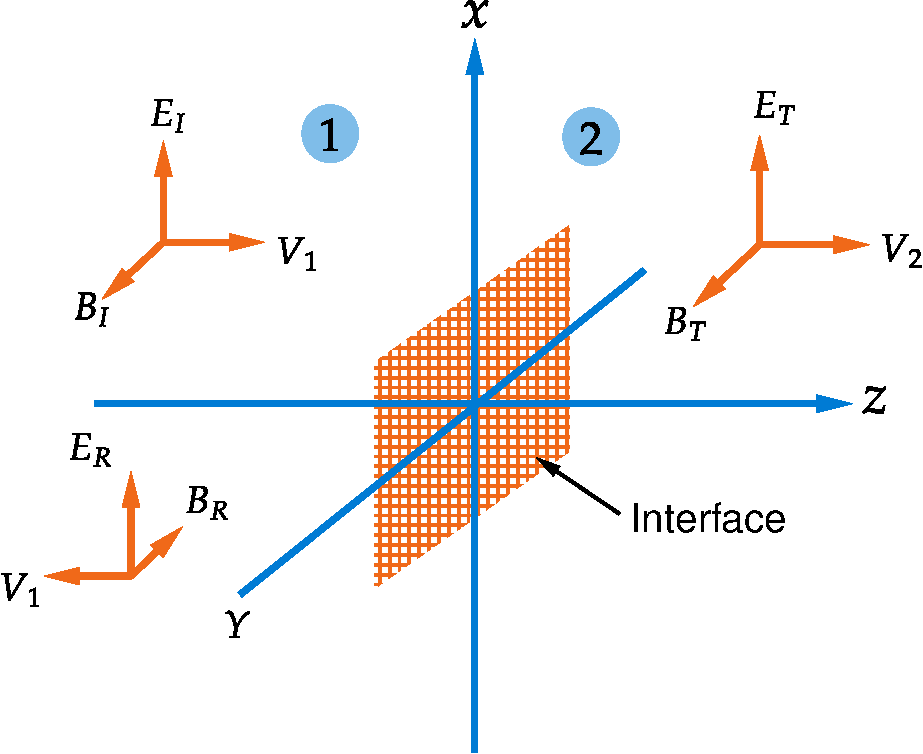
\includegraphics[height=6cm,width=8cm]{em wave}
	\caption{Reflection and Transmission at Normal incidence}
	\label{Reflection and Transmission at Normal incidence}
\end{figure}
Suppose the $xy$ plane forms the boundary between two linear media. A plane wave of frequency($\omega$)travelling in the $z$direction and polarized in $x$ direction approaches the interface from the left.

\begin{align}
\intertext{\textbf{Incident wave :}}
\left.\begin{array}{l}\vec{\mathbf{E}}_{I}(z, t)=\vec{E}_{0_{I}} e^{i\left(k_{1} z-\omega t\right)} \hat{{i}} \\\\ \vec{\mathbf{B}}_{I}(z, t)=\frac{1}{v_{1}} \vec{E}_{0_{I}} e^{i\left(k_{1} z-\omega t\right)} \hat{{j}}\end{array}\right\}\\
\notag v_1 =\text{Velocity in first medium}&\\
\intertext{\textbf{Reflected wave :}}
\left.\begin{array}{l}
\vec{\mathbf{E}}_{R}(z, t)=\vec{E}_{0_{R}} e^{i\left(-k_{1} z-\omega t\right)} \hat{{i}} \\\\
\vec{\mathbf{B}}_{R}(z, t)=-\frac{1}{v_{1}} \vec{E}_{0_{R}} e^{i\left(-k_{1} z-\omega t\right)} \hat{{j}}
\end{array}\right\}
\intertext{\textbf{Transmitted wave :}}
\left.\begin{array}{l}
\vec{\mathbf{E}}_{T}(z, t)=\vec{E}_{0_{T}} e^{i\left(k_{2} z-\omega t\right)} \hat{{i}} \\\\
\vec{\mathbf{B}}_{T}(z, t)=\frac{1}{v_{2}} \vec{E}_{0_{T}} e^{i\left(k_{2} z-\omega t\right)} \hat{{j}}
\end{array}\right\}\\
\notag v_2 =\text{Velocity in second medium}&
\end{align}
\begin{align}
\intertext{At $z=0$, the combined field on the left $\vec{E}_{I}+\vec{E}_{R}$ and $\tilde{B}_{I}+\vec{B}_{R}$, must join the fields on the
	right $\vec{E}_{T} \& \vec{B}_{T}$, in accordance with the boundary conditions in section \ref{boundary condition1}.}
\intertext{There are no electric components in perpendicular direction,Then the third boundary condition $E^\parallel_1= E^\parallel_2$ \ gives,}
\vec{E_0}_1+\vec{E_0}_R&=\vec{E_0}_T \label{waves2}
\intertext{Then the fourth boundary condition $ \frac{1}{\mu_{1}}B^\parallel_1=  \frac{1}{\mu_{2}}B^\parallel_2$ \ gives,}
\frac{1}{\mu_{1}}\left( \frac{1}{v_1}\vec{E_0}_I-\frac{1}{v_1}\vec{E_0}_R\right) &=\frac{1}{\mu_{2}}\left( \frac{1}{v_1}\vec{E_0}_I-\frac{1}{v_2}\vec{E_0}_T\right)\label{waves1}
\end{align}
\begin{align}
\notag \text{Since}\quad\vec{B_0}_I&=\frac{1}{v_1}\vec{E_0}_I\quad :\quad
\vec{B_0}_R=\frac{1}{v_1}\vec{E_0}_R\quad :\quad
\vec{B_0}_T=\frac{1}{v_2}\vec{E_0}_T\\\notag
n_2&=\frac{c}{v_2}\qquad \text{and }\qquad
n_1=\frac{c}{v_1}
\intertext{Then the equation.\ref{waves1} \ becomes,}
\vec{E_0}_1-\vec{E_0}_R&=\beta\vec{E_0}_T \label{waves3}\\
\notag \text{Where, }\qquad \beta&\equiv\frac{\mu_{1}v_1}{\mu_{2}v_2}=\frac{\mu_{1}n_2}{\mu_{2}n_1}
\intertext{By solving equation.\ref{waves2} and equation. \ref{waves3} we will get,}\notag
\vec{E_0}_R&=\left( \frac{1-\beta}{1+\beta}\right) \vec{E_0}_I \quad:\quad
\vec{E_0}_T=\left( \frac{2}{1+\beta}\right) \vec{E_0}_I
\intertext{If $\mu_{1}=\mu_{2}=\mu_{0} \Rightarrow \quad \beta=\frac{v_{1}}{v_{2}}=\frac{n_{2}}{n_{1}}$ (For non-magnetic medium). Then,}
\vec{E_0}_R&=\left( \frac{v_2-v_1}{v_1+v_2}\right) \vec{E_0}_I \quad:\quad
\vec{E_0}_T=\left( \frac{2v_2}{v_1+v_2}\right) \vec{E_0}_I
\end{align}
\begin{align}
\intertext{The reflected wave $\tilde{E_0}_R$ are in phase with incident wave if $v_2>v_1$ and out of phase if $v_2<v_1$},
\therefore {E_0}_R&=\left| \frac{v_2-v_1}{v_1+v_2}\right| {E_0}_I\quad:\quad {E_0}_T=\left(\frac{2v_2}{v_1+v_2} \right) {E_0}_I
\intertext{In terms of reflective indices $n_1$and $n_2$}
{E_0}_R&=\left| \frac{n_1-n_2}{n_1+n_2}\right| {E_0}_I\quad:\quad {E_0}_T=\left(\frac{2n_1}{n_1+n_2} \right) {E_0}_I
\intertext{Reflection coefficient,the function of incident is reflected can be find out,}
R&=\frac{I_R}{I_I}
\intertext{The intensity in general can be written as}
I&=\frac{1}{2}\varepsilon v E_0^2
\intertext{if \ $ \mu_{1}=\mu_{2}=\mu_{0} $ the \textbf{Reflection coefficient},}
R&=\frac{({E_0}_R)^2}{({E_0}_I)^2}=\left(\frac{n_1-n_2}{n_1+n_2} \right)^2  
\intertext{And \textbf{Transmission coefficient},}
T&=\frac{I_I}{I_I}=\frac{\varepsilon_2v_2}{\varepsilon_1v_1}\frac{({E_0}_I)^2}{({E_0}_I)^2}=\frac{4n_1n_2}{(n_1+n_2)^2}
\intertext{And from these equations we can show that $R+T=1$ ie. energy is conserved.}\notag
\end{align}
\hspace{5.10cm}\framebox{
	
	\parbox[t][5cm]{4.5cm}{
		
		\addvspace{0.2cm} \centering 
		\begin{align*}
		R&=\left(\frac{n_1-n_2}{n_1+n_2} \right)^2 \\\\
		T&= \frac{4n_1n_2}{(n_1+n_2)^2}\\\\
		&R+T=1
		\end{align*}
	} 
}

\begin{note}\\\vspace{0.5cm}
	When light passes from air $(n_1=1)$ and to glass$(n_2=1.5)$
	\begin{align*}
	R&=0.04,\quad4\%\\
	T&=0.96, \quad96\%
	\intertext{Most of the light are transmitted.}
	\end{align*}
\end{note}
\subsection{Reflection and transmission at oblique incidence}
\begin{figure}[H]
	\centering
	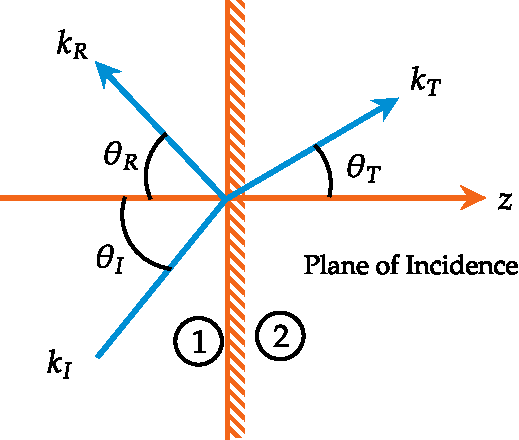
\includegraphics[height=4cm,width=6cm]{diagram-20211230-crop}
	\caption{}
	\label{}
\end{figure}
Suppose the light is travelling from $-z$ axis.There is a medium at xy plane.Light get reflected and transmitted from the plane.suppose the incident light make an angle $\theta_I$ with the normal ie z axis.Let $\omega$ be the frequency of the travelling wave.\\
\textbf{Incident wave:}
$$E_I(r,t)=E_{0I}e^{(k_I.r-\omega t)}$$
$$B_{I}(r,t)=\frac{1}{v_1}(k_I\times E_I)$$
\textbf{Reflected wave:}
$$E_R(r,t)=E_{0R}e^{(k_R.r-\omega t)}$$
$$B_{R}(r,t)=\frac{1}{v_1}(k_R\times E_R)$$
Where $v_1$ be the velocity of first medium.\\
\textbf{Transmitted wave}
$$E_T(r,t)=E_{0T}e^{(k_T.r-\omega t)}$$
$$B_{T}(r,t)=\frac{1}{v_2}(k_T\times E_T)$$
Where $v_2$ be the velocity of the second medium.\\
The frequency of all the waves are same.so we can relate,\\
$$k_Iv_1=k_Rv_1=k_Tv_2$$
$$\implies k_I=k_R$$
$$\implies k_I=k_R=\frac{v_2}{v_1}k_T=\frac{n_1}{n_2}k_T$$
Where $n_1$ and $n_2$ are the refractive index of the first and second medium.\\
At $z=0$ the combined field of electric and magnetic components  are equal\\
ie $$E_I+E_R=E_T$$ and 
$$B_I+B_R=B_T$$
Which give rise to\\
$$E_I(r,t)=E_{0I}e^{(k_I.r-\omega t)}+E_R(r,t)=E_{0R}e^{(k_R.r-\omega t)}=E_T(r,t)=E_{0T}e^{(k_T.r-\omega t)}$$
Because the boundary conditions must hold at all points on the plane and for all time ,these exponential factors must be equal at z=0.Which implies\\
$$k_I\cdot r=k_R\cdot r=k_T\cdot r \quad at z=0$$
after taking the dot product\\
$$x(k_I)_x+y(k_I)_y=x(k_R)_x+y(k_R)_y=x(k_T)_x+y(k_T)_y$$
\textbf{if x=0}
$$(k_I)_y=(k_R)_y=(k_T)_y$$
suppose the incident ray lies in the xz plane then $(k_I)_y=0$\\
Then$$(k_R)_y=(k_T)_y=0$$
There will be no ray along y axis.
Which means that all the rays lies in the same plane.\\
conclusion\\
\textbf{First law}:The incident ,reflected, and transmitted wavevectors form a plane.(called plane of incidence),which also include the normal to the surface(z axix)\\
Here the common plane is xz plane\\
\textbf{if y=o}\\
$$(k_I)_x=(k_R)_x=(k_T)_x$$
Which implies that 
$$k_I\sin \theta_I=k_R\sin\theta_R=k_T\sin \theta_T$$
Where $\theta_I$ is the angle of incidence,$\theta_R$ is the angle of reflection,and $\theta_T$ is called angle of transmission also known as angle of refraction.\\
\textbf{Second law}
$$k_I\sin \theta_I=k_R\sin\theta_R$$
$$k_I=k_R$$
Then $$\theta_I=\theta_R$$
The angle of incidence is the angle of reflection
$$k_I=k_R\neq k_T$$
Then  $$\frac{\sin \theta_I}{\sin \theta_T}=\frac{k_T}{k_R}$$
\paragraph{Third law}
$$\frac{\sin \theta_I}{\sin \theta_T}=\frac{n_1}{n_2}$$
This is the \textbf{law of refraction or Snell's law.}
\subsection{Polarization}
Consider the boundary conditions at the surface\\
$$(i)\quad \epsilon_{1}(E_{0_I}+E_{0_R})_z=\epsilon_{2}(E_{0_T})_z$$
$$ (ii) \quad (B_{O_I}+B_{0_R})_z=(B_{0_T})_z$$
$$(iii) \quad (E_{0_I}+E_{0_R})_{x,y}=(E_{0_T})_{x,y}$$
$$(iv) \quad \frac{1}{\mu_{1}}(B_{0_I}+B_{0_R})_{x,y}=\frac{1}{\mu_{2}}(B_{0_T})_{x,y}$$
Suppose the polarization of the incident wave is parallel to the plane of incidenceie in the xz plane.\\
Consider the first boundary condition\\
$$\epsilon_{1}(-E_{0_I}\sin \theta_I+E_{0_R}\sin \theta_R)=\epsilon_{2}(-E_{0_T}\sin \theta_T)$$
Since magnetic field has no z components (ii) add nothing.\\
(iii)equation become\\
$$E_{0_I}\cos \theta_I+E_{0_R}\cos \theta_R=E_{0_T}\cos \theta_T$$\\
(iv) Become\\
$$\frac{1}{\mu_{1} v_1}(E_{0_I}-E_{0_R})=\frac{1}{\mu_{2} v_2}E_{0_T}$$
Combining with $\epsilon_{1}(-E_{0_I}\sin \theta_I+E_{0_R}\sin \theta_R)=\epsilon_{2}(-E_{0_T}\sin \theta_T)$ and using laws of reflection and refraction,we will get
$$E_{0_I}-E_{0_R}=\beta E_{0_T}$$
Where $$\beta= \frac{\mu_{1} v_1}{\mu_{2} v_2}=\frac{\mu_{1} n_2}{\mu_{2}n_1}$$
Equation $$E_{0_I}\cos \theta_I+E_{0_R}\cos \theta_R=E_{0_T}\cos \theta_T$$
$$E_{0_I}+E_{0_R}=\alpha E_{0_T}$$
Where $$\alpha=\frac{\cos \theta_T}{\cos \theta_I}$$\\
solving $E_{0_I}+E_{0_R}=\alpha E_{0_T}$, \quad $E_{0_I}-E_{0_R}=\beta E_{0_T}$ this equation for reflected and transmitted amplitude we obtain\\
Amplitude of reflected wave is\\
$$E_{0_R}=\frac{\alpha-\beta}{\alpha+\beta}E_{0_I}$$
Amplitude of the transmitted wave is\\
$$E_{0_T}=\left( \frac{2}{\alpha+\beta}\right)E_{0_I} $$
These are known as \textbf{Fresnel's equations}\\
\begin{note}
	The transmitted wave is always in phase with the incident one;reflected wave is either in phase if $\alpha>\beta$ or 180 out of phase if $\alpha< \beta$
\end{note}
The amplitude of the transmitted and reflected wave depends on the angle of incidence because $\alpha$ is a function of $\theta_I$
$$\alpha=\frac{\sqrt{1-\sin ^{2} \theta_{T}}}{\cos \theta_{I}}=\frac{\sqrt{1-\left[\left(n_{1} / n_{2}\right) \sin \theta_{I}\right]^{2}}}{\cos \theta_{I}}$$
\paragraph{Brewster's angle}
At normal incidenace most of the light are transmitted.At $\theta_I=90^{\circ}$ the wave is totally reflected.Between these two angle there is some angle called Brewster's angle at which the reflected ray is completely disappered.\\
\begin{figure}[H]
	\centering
	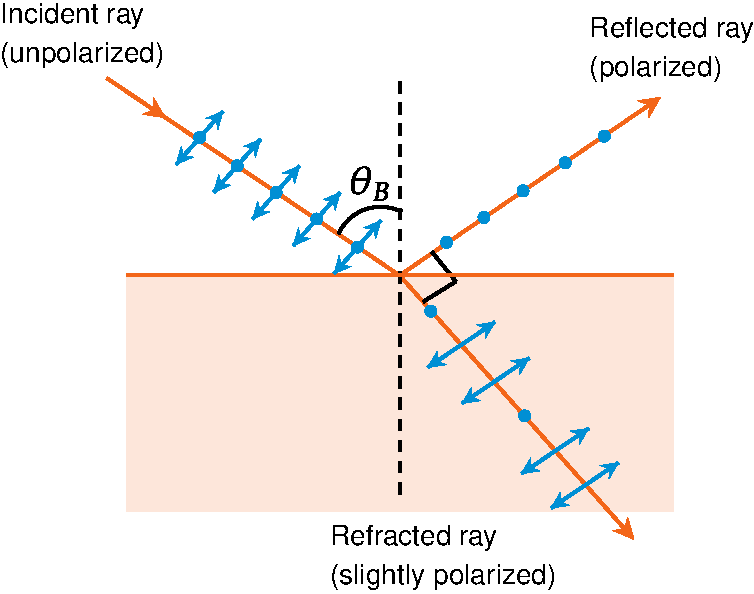
\includegraphics[height=6cm,width=8cm]{diagram-20211216-crop}
	\caption{}
	\label{}
\end{figure}
This occurs when $\alpha=\beta$\\
$$\sin ^{2} \theta_{B}=\frac{1-\beta^{2}}{\left(n_{1} / n_{2}\right)^{2}-\beta^{2}}$$
For the typical case $\mu_{1}\approx\mu_{2}$ so $\beta \approx n_2, \sin^2 \theta_{B}\approx \frac{\beta^2}{1+\beta^2}$ and hence\\
$$\tan \theta_{B} \approx \frac{n_2}{n_1}$$
\begin{note}
	If the incident light is unpolarized the reflected ray will be totally polarized parallel to the interface at Brewster's angle.In the above condition we use plane polarized light as incident light,that is why there is no reflected rays.
\end{note}
\textbf{ Malus law }\\
	\textbf{The power per unit area}
\begin{note}
	\begin{enumerate}
		\item Incident intensity\\
		$$I_I=\frac{1}{2}\epsilon_{1}v_1E_{0_I}^2 \cos \theta_{I}$$
		\item Reflected intencity
		$$I_R=\frac{1}{2}\epsilon_{1}v_1E_{0_R}^2 \cos \theta_{R}$$
		\item Transmitted intencity
		$$I_T=\frac{1}{2}\epsilon_{2}v_2E_{0_T}^2 \cos \theta_{T}$$
	\end{enumerate}
\end{note}
\textbf{Reflection and transmission coefficient}
$$R=\frac{I_R}{I_I}=\left( \frac{E_{0_R}}{E_{O_I}}\right) =\left( \frac{\alpha-\beta}{\alpha+\beta}\right) ^2$$
$$T=\frac{I_T}{I_I}=\frac{\epsilon_{2}v_2}{\epsilon_{1}v_1}\left( \frac{E_{0_T}}{E_{0I}}\right) \frac{\cos \theta_{T}}{\cos \theta_{I}}=\alpha \beta\left( \frac{2}{\alpha+\beta} \right) ^2$$
\section{Elctromagnetic waves in conductors}
When we are talking about wave propagation through a vacuum or through a dielctric mterial we restricted our assumption that $J_f$ and $\rho_f$ are zeros.But in the case of conductors we donnot independently control the flow of charge, and in general $J_f$ is not certainly zero.\\
According to ohm's law the current density in a conductor is proportional to the electric field.\\
$$J_f=\sigma E$$
Maxwell' equation for a linear media.\\
(i)\quad $\nabla$ $\cdot$ E=$\frac{\rho_f}{\epsilon}$\\
(ii) \quad $\nabla \cdot B=0$\\
(iii)\quad $\nabla$ $\times$ =-$\frac{\partial B}{\partial t}$\\
(iv) \quad $\nabla \times B=\mu \sigma E+\mu \epsilon \frac{\partial E}{\partial t}$\\
Continuity equation ($\nabla \cdot J_f=\frac{\partial \rho_f}{\partial t}$) with Ohm's law The gauss's law become\\
$$\frac{\partial \rho_f}{\partial t}=-\sigma (\nabla \cdot E)=-\frac{\sigma}{\epsilon}\rho_f$$
$$\rho_f(t)=e^{\frac{-\sigma}{\epsilon}t} \rho_f(0)$$
which means that if you put some charges on a conductor,it will flow out of the edges.Donot mind this transient behaviour.consider the time up to which the accumulated free charges to disappear.From then $\rho_f=0$\\
Now maxwell's quations become\\
(i)\quad $\nabla$ $\cdot$ E=0\\
(ii) \quad $\nabla \cdot B=0$\\
(iii)\quad $\nabla$ $\times$ =-$\frac{\partial B}{\partial t}$\\
(iv) \quad $\nabla \times B=\mu \sigma E+\mu \epsilon \frac{\partial E}{\partial t}$\\
Applying curl to (iii) and (iv) we will get modified wave equation for E and B.\\
$$\nabla^{2} \mathbf{E}=\mu \epsilon \frac{\partial^{2} \mathbf{E}}{\partial t^{2}}+\mu \sigma \frac{\partial \mathbf{E}}{\partial t}, \quad \nabla^{2} \mathbf{B}=\mu \epsilon \frac{\partial^{2} \mathbf{B}}{\partial t^{2}}+\mu \sigma \frac{\partial \mathbf{B}}{\partial t}$$
These equations still admit plane-wave solutions,
$$
\tilde{\mathbf{E}}(z, t)=\tilde{\mathbf{E}}_{0} e^{i(k z-\omega t)}, \quad \tilde{\mathbf{B}}(z, t)=\tilde{\mathbf{B}}_{0} e^{i(\tilde{k} z-\omega t)},
$$
but this time the "wave number" $\tilde{k}$ is complex:
$$
\tilde{k}^{2}=\mu \epsilon \omega^{2}+i \mu \sigma \omega,
$$
$$\bar{k}=k_{real}+ik_{img}$$
where
$$
k_{real} \equiv \omega \sqrt{\frac{\epsilon \mu}{2}}\left[\sqrt{1+\left(\frac{\sigma}{\epsilon \omega}\right)^{2}}+1\right]^{1 / 2}
$$
and 
$$k_{img} \equiv \omega \sqrt{\frac{\epsilon \mu}{2}}\left[\sqrt{1+\left(\frac{\sigma}{\epsilon \omega}\right)^{2}}-1\right]^{1 / 2}$$
Now\\
$$\tilde{\mathbf{E}}(z, t)=\tilde{\mathbf{E}}_{0} e^{-k_{real} z} e^{i(k_{img} z-\omega t)}, \quad \tilde{\mathbf{B}}(z, t)=\tilde{\mathbf{B}}_{0} e^{-k_{real}z} e^{i(k_{imag} z-\omega t)}$$
\paragraph{Skin depth}
The distance it takes to reduce the amplitude by a factor of $1 / e$ (about a third) is called the skin depth:
$$
d \equiv \frac{1}{\kappa}
$$
it is a measure of how far the wave penetrates into the conductor. Meanwhile, the real part of $k$ determines the wavelength, the propagation speed, and the index of refraction, in the usual way:
$$
\lambda=\frac{2 \pi}{k}, \quad v=\frac{\omega}{k}, \quad n=\frac{c k}{\omega} .
$$
\subsection{ Skin depth in a poor conductor:}
For poor conductor
$$
\begin{gathered}
\sigma \ll \omega \epsilon \\
\kappa \equiv \omega \sqrt{\frac{\epsilon \mu}{2}}\left[\sqrt{1+\left(\frac{\sigma}{\epsilon \omega}\right)^{2}}-1\right]^{1 / 2} \\
\approx \omega \sqrt{\frac{\epsilon \mu}{2}}\left[1+\frac{1}{2}\left(\frac{\sigma}{\epsilon \omega}\right)^{2}-1\right]^{1 / 2}
\end{gathered}
$$
Then
$$
\kappa \approx \omega \sqrt{\frac{\epsilon \mu}{2} \frac{1}{\sqrt{2}} \frac{\sigma}{\epsilon \omega}}=\frac{\sigma}{2} \sqrt{\frac{\mu}{\epsilon}}
$$
So
$$
d=\frac{1}{\kappa} \cong \frac{2}{\sigma} \sqrt{\frac{\epsilon}{\mu}}
$$
\subsection{ Skin depth in a good conductor:}
For good conductor
$$
\sigma \gg \omega \epsilon
$$
$$
\begin{aligned}
\kappa & \equiv \omega \sqrt{\frac{\epsilon \mu}{2}}\left[\sqrt{\left.1+\left(\frac{\sigma}{\epsilon \omega}\right)^{2}-1\right]^{1 / 2}}\right.\\
& \approx \omega \sqrt{\frac{\epsilon \mu}{2}\left(\frac{\sigma}{\epsilon \omega}\right)^{1 / 2}} \approx \sqrt{\frac{\mu \sigma \omega}{2}}
\end{aligned}
$$
So for a good conductor
$$
d \cong \sqrt{\frac{2}{\mu \sigma \omega}}
$$
For good conductor as $\sigma \gg \omega \epsilon$ so, you can see
$$
k \cong \kappa
$$
or
$$
\lambda=\frac{2 \pi}{k} \cong \frac{2 \pi}{\kappa}=2 \pi d, \text { or } d=\frac{\lambda}{2 \pi}
$$
\textbf{Phase shift}\\
Like any complex number, $\tilde{k}$ can be expressed in terms of its modulus and phase:
$$
\tilde{k}=K e^{i \phi},
$$
$$\begin{gathered}
K \equiv|\tilde{k}|=\sqrt{k_{real}^{2}+k_{img}^{2}}=\omega \sqrt{\epsilon \mu \sqrt{1+\left(\frac{\sigma}{\epsilon \omega}\right)^{2}}} \\
\phi \equiv \tan ^{-1}(k_{img} / k_{real})
\end{gathered}$$
 The complex amplitudes $\tilde{E}_{0}=E_{0} e^{i \delta_{E}}$ and $\tilde{B}_{0}=B_{0} e^{i \delta_{B}}$ are related by
$$
B_{0} e^{i \delta_{B}}=\frac{K e^{i \phi}}{\omega} E_{0} e^{i \delta_{E}}
$$
Evidently the electric and magnetic fields are no longer in phase; in fact,
$$
\delta_{B}-\delta_{E}=\phi
$$
the magnetic field lags behind the electric fleld. Meanwhile, the (real) amplitudes of $\mathbf{E}$ and B are related by
$$
\frac{B_{0}}{E_{0}}=\frac{K}{\omega}=\sqrt{\epsilon \mu \sqrt{1+\left(\frac{\sigma}{\epsilon \omega}\right)^{2}}} .
$$
The (real) electric and magnetic fields are, finally,
$$
\left.\frac{\mathbf{E}(z, t)=E_{0} e^{-\kappa z} \cos \left(k z-\omega t+\delta_{E}\right) \hat{\mathbf{x}},}{\mathbf{B}(z, t)=B_{0} e^{-\kappa z} \cos \left(k z-\omega t+\delta_{E}+\phi\right) \hat{\mathbf{y}}}\right\}$$
\begin{exercise}
 (a) Find the skin depth of pure water. You are given that for pure water conductivity $\sigma=1 /\left(2.5 \times 10^{5}\right)$, dielectric constant $k=80.1$ and $\mu \approx \mu_{0}$.\\
 (b) Find the skin depth (in nanometers) for a typical metal whose conductivity $\sigma \approx 10^{7}$, the frequency $\omega \approx 10^{15}$ with $\epsilon \approx \epsilon_{0}$ and $\mu \approx \mu_{0}$.
\end{exercise}
\begin{answer}
 (a) Conductivity shows that the water is a poor conductor. Hence we will take approximation $d=\frac{1}{\kappa} \cong$ $\frac{2}{\sigma} \sqrt{\frac{\epsilon}{\mu}} .$
$$
d=(2)\left(2.5 \times 10^{5}\right) \sqrt{\frac{(80.1)\left(8.85 \times 10^{-12}\right)}{4 \pi \times 10^{-7}}}=1.19 \times 10^{4} \mathrm{~m}
$$
(b) We have proved that for good conductor $d \approx \sqrt{\frac{2}{\mu \sigma \omega}}$. Put the values to get
$$
d=\frac{1}{8 \times 10^{7}}=1.3 \times 10^{-8}=13 \mathrm{~nm}
$$
So the fields do not penetrate far into a metal	
\end{answer}
\subsection{Reflection at a conducting surface}
Boundary conditions used to solve em waves at the conductor involves $\rho_f$ and $K_f$\\
(i) $\epsilon_{1} E_{1}^{\perp}-\epsilon_{2} E_{2}^{\perp}=\sigma_{f}$,\\
(iii) $\mathbf{E}_{1}^{\|}-\mathbf{E}_{2}^{\|}=0$,\\
(ii) $B_{1}^{\perp}-B_{2}^{\perp}=0$,\\
(iv) $\frac{1}{\mu_{1}} \mathbf{B}_{1}^{\|}-\frac{1}{\mu_{2}} \mathbf{B}_{2}^{\|}=\mathbf{K}_{f} \times \hat{\mathbf{n}}$,\\
Suppose that xy plane forms a boundary between a non conducting non linear medium 1 and a conductor 2.A monochromatic plane wave travelling in the z direction and polarized in the x direction ,approches from the left as shown in figure.\\
\begin{figure}[H]
	\centering
	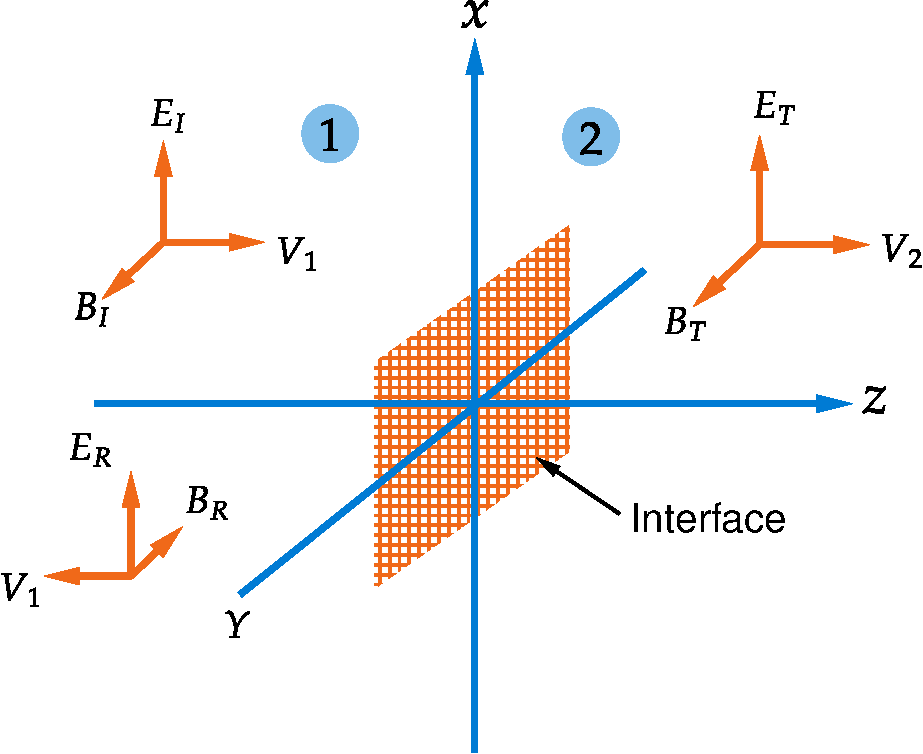
\includegraphics[height=6cm,width=8cm]{em wave}
	\caption{Reflection and Transmission at Normal incidence}
	\label{Reflection and Transmission at Normal incidence}
\end{figure}
\textbf{Incident wave:}
$$\tilde{\mathbf{E}}_{I}(z, t)=\tilde{E}_{0_{I}} e^{i\left(k_{1} z-\omega t\right)} \hat{\mathbf{x}}$$
$$ \quad \tilde{\mathbf{B}}_{I}(z, t)=\frac{1}{v_{1}} \tilde{E}_{0_{I}} e^{i\left(k_{1} z-\omega t\right)} \hat{\mathbf{y}}$$
\textbf{Reflected wave:}
$$\tilde{\mathbf{E}}_{R}(z, t)=\tilde{E}_{0_{R}} e^{i\left(-k_{1} z-\omega t\right)} \hat{\mathbf{x}}$$
$$ \quad \tilde{\mathbf{B}}_{R}(z, t)=-\frac{1}{v_{1}} \tilde{E}_{0_{R}} e^{i\left(-k_{1} z-\omega t\right)} \hat{\mathbf{y}}$$
\textbf{Transmitted wave:}
$$\tilde{\mathbf{E}}_{T}(z, t)=\tilde{E}_{0_{T}} e^{i\left(\tilde{k}_{2} z-\omega t\right)} \hat{\mathbf{x}}$$
$$ \quad \tilde{\mathbf{B}}_{T}(z, t)=\frac{\tilde{k}_{2}}{\omega} \tilde{E}_{0_{T}} e^{i\left(\tilde{k}_{2} z-\omega t\right)} \hat{\mathbf{y}}$$
Transmitted wave will get attinuated while entering the conducting material.\\
Now consider the boundary conditions one by one.\\
(i) Gives $\sigma_{f}=0$ because there will be no perpendicular component of elctric field in two media($E^{\perp}$)=0\\
(ii)yields $B^{\perp}=0$\\
(iii) gives $$\tilde{E}_{0_{1}}+\tilde{E}_{0_{R}}=\tilde{E}_{0_{\tau}}$$
(iv) gives $$\begin{gathered}
\frac{1}{\mu_{1} v_{1}}\left(\tilde{E}_{0_{l}}-\tilde{E}_{0_{R}}\right)-\frac{\tilde{k}_{2}}{\mu_{2} \omega} \tilde{E}_{0_{T}}=0, \\
\tilde{E}_{0_{I}}-\tilde{E}_{0_{R}}=\tilde{\beta} \tilde{E}_{0_{T}}, \\
\tilde{\beta} \equiv \frac{\mu_{1} v_{1}}{\mu_{2} \omega} \tilde{k}_{2} .
\end{gathered}$$
It follows that
$$
\tilde{E}_{0_{R}}=\left(\frac{1-\tilde{\beta}}{1+\tilde{\beta}}\right) \tilde{E}_{0_{l}}, \quad \tilde{E}_{0_{T}}=\left(\frac{2}{1+\tilde{\beta}}\right) \tilde{E}_{0_{l}} .
$$
For a perfect conductor ($\sigma=\inf$),$k_2=\infty$ so $\beta$ is finite and \\
$$E_{0_R}=-E_{0_I}, \quad E_{0_T}=0$$
In this case the wave is totally reflected with a $180^{\circ}$ phase shift.That is why excellent conductors make good mirrors.
\section{Guided waves}
Untill now we have dealt with plane wave of infinite extent;Now we consider the em waves confines to the interior of a hollow pipe or wave guide.We will assume the wave guide is perfect conductor. so that E=0 and B=0 inside the material itself.Hence the boundary conditions at the boundary wall are\\
$$ (i) \quad  E^{\parallel}=0$$ 
$$ (ii) \quad B^{\perp}=0$$
\begin{figure}[H]
	\centering
	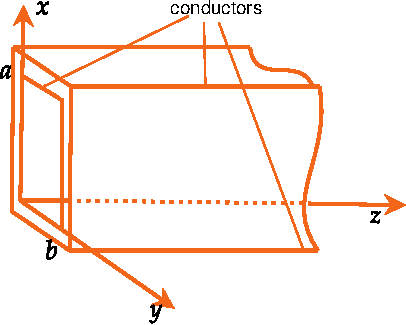
\includegraphics[height=5cm,width=8cm]{wave guide 2-crop}
	\caption{}
	\label{}
\end{figure}
Let us take the medium is restricted by $x$ and $y$ and the wave is propagating along $z$ direction.So E and B has the generic form.\\
$$(i) \tilde{\mathbf{E}}(x, y, z, t)=\tilde{\mathbf{E}}_{0}(x, y) e^{i(k z-\omega t)}$$
$$(ii) \tilde{\mathbf{B}}(x, y, z, t)=\tilde{\mathbf{B}}_{0}(x, y) e^{i(k z-\omega t)}$$
The maxwell's equation in the interior of the waveguide\\
$$(i) \boldsymbol{\nabla} \cdot \mathbf{E}=0$$
$$(ii)\boldsymbol{\nabla} \cdot \mathbf{B}=0$$
$$(iii) \nabla \times \mathbf{E}=-\frac{\partial \mathbf{B}}{\partial t}$$
$$(iv) \boldsymbol{\nabla} \times \mathbf{B}=\frac{1}{c^{2}} \frac{\partial \mathbf{E}}{\partial t}$$
 Boundary conditions and the Maxwell's equations gives \\
$$ (i) \left[\frac{\partial^{2}}{\partial x^{2}}+\frac{\partial^{2}}{\partial y^{2}}+(\omega / c)^{2}-k^{2}\right] E_{z}=0$$ and\\
$$ (ii) \left[\frac{\partial^{2}}{\partial x^{2}}+\frac{\partial^{2}}{\partial y^{2}}+(\omega / c)^{2}-k^{2}\right] B_{z}=0$$
If $E_{z}=0$, we call these TE (transverse electric") waves; if $B_{z}=0$, they are called TM ("transverse magnetic") waves; if both $\mathrm{E}_{\mathrm{z}}=0$ and $\mathrm{B}_{\mathrm{z}}=0$, we call them TEM waves. You can prove that TEM waves can't occur in hollow rectangular wave guide.\\
\begin{center}
 TE, mode $\Rightarrow F_{z}=0 \quad B_{z}=$ exist\\
$\mathrm{TM}$ mode $\Rightarrow E_{z}=$ exist $B_{z}=0$\\
TEM mode $\Rightarrow E_{z}=B_{z}=0$\\	
\end{center}
\subsection{ TE Waves in a Rectangular Wave Guide}
We need the solution of
$$\text { (ii) }\left[\frac{\partial^{2}}{\partial x^{2}}+\frac{\partial^{2}}{\partial y^{2}}+(\omega / c)^{2}-k^{2}\right] B_{z}=0$$
Take $$
B_{z}(x, y)=X(x) Y(y)
$$
and do the separation of variable. You get the solution
$$
B_{z}=B_{0} \cos (m \pi x / a) \cos (n \pi y / b)
$$
with the dispersion relation
$$k=\sqrt{(\omega / c)^{2}-\pi^{2}\left[(m / a)^{2}+(n / b)^{2}\right]}$$
Define
$$
\omega_{m n}=c \pi \sqrt{(m / a)^{2}+(n / b)^{2}}
$$
Now you see if
$$
\omega<\omega_{m n}
$$
the wave number is imaginary, and instead of a traveling wave we have exponentially attenuated wave which will rapidly absorbed in the medium. $\omega_{m n}$ is called the cut off frequency for a particular mode $T E_{m n}$. You should remember that $\omega$ is angular frequency, not frequency.\\
In terms of frequency
$$
\nu_{m n}=\frac{c}{2} \sqrt{\left(\frac{m}{a}\right)^{2}+\left(\frac{n}{b}\right)^{2}}
$$
The lowest mode is TE $_{10}$ (usually among $a$ and $b$ the larger is taken to be $a$.
$$\omega_{10}=c \pi / a$$
\textbf{Group and phase velocity}\\
Phase velocity is greater than C.\\
$$v_{p}=\frac{\omega}{k}=\frac{c}{\sqrt{1-\left(\omega_{m n} / \omega\right)^{2}}}$$
The group velocity
$$
v_{g}=\frac{1}{d k / d \omega}=c \sqrt{1-\left(\omega_{m n} / \omega\right)^{2}}<c
$$
\subsection{ TM Waves in a Rectangular Wave Guide}
$$\left[\frac{\partial^{2}}{\partial x^{2}}+\frac{\partial^{2}}{\partial y^{2}}+(\omega / c)^{2}-k^{2}\right] E_{z}=0$$
Has the soltion of the form.
$$E_{z}=E_{0} \sin \left(\frac{m \pi x}{a}\right) \sin \left(\frac{n \pi y}{b}\right)$$
if either of the $m$ and $n$ is zero the solution itself is zero. So the lowest frequency mode is for TM wave in rectangular wave guide is $T E_{11}$.\\
\section{Resonant cavity}
Resonant cavity produced by closing off the two ends of a rectangular wave guide, at $z=0$ and at $z=d$, making a perfectly conducting empty box.\\
\begin{figure}[H]
	\centering
	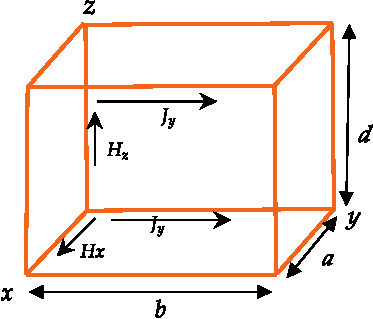
\includegraphics[height=5cm,width=8cm]{resonant-crop}
	\caption{}
	\label{}
\end{figure}
We can prove that the cut off frequencies for both $\mathrm{TE}$ and TM modes in a resonance cavity are given by
$$\begin{gathered}
\omega_{l m n}=c \pi \sqrt{(l / d)^{2}+(m / a)^{2}+(n / b)^{2}} \\
\nu_{l m n}=\frac{c}{2} \sqrt{(l / d)^{2}+(m / a)^{2}+(n / b)^{2}}
\end{gathered}$$
\begin{exercise}
	 What should be the 3rd dimension of a cavity of cross section $1 \mathrm{~cm} \times 1 \mathrm{~cm}$ which operates at $T E_{103}$ mode at $24 \mathrm{GHz} ? ?$
\end{exercise}
\begin{answer}
Solution: $l=1, m=0, n=3$. use
$$
\nu_{103}=24 \times 10^{9} ; \quad a=0.01, b=0.01, c=?
$$
use the formula of $\nu_{l m n}$ to get
$$\nu_{l m n}=\frac{c}{2} \sqrt{(l / d)^{2}+(m / a)^{2}+(n / b)^{2}}$$
$$
\left(\frac{24 \times 2 \times 10^{9}}{3 \times 10^{8}}\right)^{2}=\left(\frac{1}{0.01}\right)^{2}+0+\left(\frac{3}{c}\right)^{2}
$$
$$c=0.02$$	
\end{answer}
\section{ Dielectric inserted into waveguide}
When there is a dielectric / magnetic medium inside of a dielectric instead of vacuum, just replace $c$ by $\frac{1}{\sqrt{\epsilon \mu}}$
$$\nu_{m n}=\frac{1}{2 \sqrt{\epsilon \mu}} \sqrt{\left(\frac{m}{a}\right)^{2}+\left(\frac{n}{b}\right)^{2}}$$
For most of the material $\mu \approx \mu_{0}$, so then
$$
\begin{aligned}
\nu_{m n} &=\frac{1}{2 \sqrt{\epsilon_{r}} \epsilon_{0} \mu_{0}} \sqrt{\left(\frac{m}{a}\right)^{2}+\left(\frac{n}{b}\right)^{2}} \\
&=\frac{c}{2 \sqrt{\epsilon_{r}}} \sqrt{\left(\frac{m}{a}\right)^{2}+\left(\frac{n}{b}\right)^{2}}
\end{aligned}
$$
\begin{exercise}
 For a air filled wave guide. the cut off frequency $T E_{0}=1.8756 \mathrm{GHz}$. What will be the cut off frequency if one dielectric of relative permeability $\epsilon=9 \epsilon_{0}$ is inserted in the dielectric?
\end{exercise}
\begin{answer}
 you have already derived the formula for cut off frequency for the dielectric inserted wave guide. The ans is
$$
\nu_{m n}^{\text {dielectric }}=\nu_{m n}^{\text {vacuum }} / \sqrt{\epsilon_{r}}=1.8756 / 3 \mathrm{GHz}
$$	
\end{answer}
\newpage
\begin{abox}
	Practice set 1
	\end{abox}
\begin{enumerate}
\begin{minipage}{\textwidth}
	\item A plane electromagnetic wave is propagating in a lossless dielectric. The electric field is given by
	$$
	\vec{E}(x, y, z, t)=E_{0}(\hat{x}+A \hat{z}) \exp \left[i k_{0}\{-c t+(x+\sqrt{3} z)\}\right]
	$$
	where $c$ is the speed of light in vacuum, $E_{0}, A$ and $k_{0}$ are constant and $\hat{x}$ and $\hat{z}$ are unit vectors along the $x$-and $z$-axes. The relative dielectric constant of the medium $\varepsilon_{r}$ and the constant $A$ are
	\exyear{NET JUNE 2011}
\end{minipage}
\begin{tasks}(2)
	\task[\textbf{A.}]$\varepsilon_{r}=4$ and $A=-\frac{1}{\sqrt{3}}$
	\task[\textbf{B.}]$\varepsilon_{r}=4$ and $A=+\frac{1}{\sqrt{3}}$
	\task[\textbf{C.}]$\varepsilon_{r}=4$ and $A=\sqrt{3}$
	\task[\textbf{D.}]$\varepsilon_{r}=4$ and $A=-\sqrt{3}$
\end{tasks}
\begin{minipage}{\textwidth}
	\item The magnetic field of the $T E_{11}$ mode of a rectangular waveguide of dimensions $a \times b$ as shown in the figure is given by $H_{z}=H_{0} \cos (0.3 \pi x) \cos (0.4 \pi y)$, where $x$ and $y$ are in cm
	\exyear{NET JUNE 2011}
	\begin{figure}[H]
		\centering
		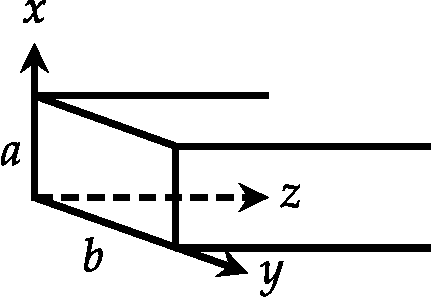
\includegraphics[height=3cm,width=5cm]{diagram-20211011(7)-crop}
	\end{figure}
\end{minipage}
$\text { A. The dimensions of the waveguide are }$
\begin{tasks}(2)
	\task[\textbf{A.}] $a=3.33 \mathrm{~cm}, b=2.50 \mathrm{~cm}$
	\task[\textbf{B.}]$a=0.40 \mathrm{~cm}, b=0.30 \mathrm{~cm}$
	\task[\textbf{C.}]$a=0.80 \mathrm{~cm}, b=0.60 \mathrm{~cm}$
	\task[\textbf{D.}] $a=1.66 \mathrm{~cm}, b=1.25 \mathrm{~cm}$
\end{tasks}

\begin{minipage}{\textwidth}
	\item An electromagnetic wave is incident on a water-air interface. The phase of the perpendicular component of the electric field, $E_{\perp}$, of the reflected wave into the water is found to remain the same for all angles of incidence. The phase of the magnetic field $H$
	\exyear{NET JUNE 2012}
\end{minipage}
\begin{tasks}(2)
	\task[\textbf{A.}]does not change
	\task[\textbf{B.}]changes by $3 \pi / 2$
	\task[\textbf{C.}]changes by $\pi / 2$
	\task[\textbf{D.}]changes by $\pi$
\end{tasks}

\begin{minipage}{\textwidth}
	\item A current $I$ is created by a narrow beam of protons moving in vacuum with constant velocity $\vec{u}$. The direction and magnitude, respectively of the Poynting vector $\vec{S}$ outside the beam at a radial distance $r$ (much larger than the width of the beam) from the axis, are
	\exyear{NET JUNE 2013}
\end{minipage}
\begin{tasks}(2)
	\task[\textbf{A.}] $\vec{S} \perp \vec{u}$ and $|\vec{S}|=\frac{I^{2}}{4 \pi^{2} \varepsilon_{0}|\vec{u}| r^{2}}$
	\task[\textbf{B.}]$\vec{S} \|(-\vec{u})$ and $|\vec{S}|=\frac{I^{2}}{4 \pi^{2} \varepsilon_{0}|\vec{u}| r^{4}}$
	\task[\textbf{C.}]$\vec{S} \| \vec{u}$ and $|\vec{S}|=\frac{I^{2}}{4 \pi^{2} \varepsilon_{0}|\vec{u}| r^{2}}$
	\task[\textbf{D.}]$\vec{S} \| \vec{u}$ and $|\vec{S}|=\frac{I^{2}}{4 \pi^{2} \varepsilon_{0}|\vec{u}| r^{4}}$
\end{tasks}
\begin{minipage}{\textwidth}
	\item The electric field of an electromagnetic wave is given by
	$$
	\vec{E}=E_{0} \cos [\pi(0.3 x+0.4 y-1000 t)] \hat{k} .
	$$
	The associated magnetic field $\vec{B}$ is
	\exyear{NET DEC 2013}
\end{minipage}
\begin{tasks}(2)
	\task[\textbf{A.}] $10^{-3} E_{0} \cos [\pi(0.3 x+0.4 y-1000 t)] \hat{k}$
	\task[\textbf{B.}]$10^{-4} E_{0} \cos [\pi(0.3 x+0.4 y-1000 t)](4 \hat{i}-3 \hat{j})$
	\task[\textbf{C.}]$E_{0} \cos [\pi(0.3 x+0.4 y-1000 t)](0.3 \hat{i}+0.4 \hat{j})$
	\task[\textbf{D.}]$10^{2} E_{0} \cos [\pi(0.3 x+0.4 y-1000 t)](3 \hat{i}+4 \hat{j})$
\end{tasks}
\begin{minipage}{\textwidth}
	\item A beam of light of frequency $\omega$ is reflected from a dielectric-metal interface at normal incidence. The refractive index of the dielectric medium is $n$ and that of the metal is $n_{2}=n(1+i \rho)$. If the beam is polarised parallel to the interface, then the phase change experienced by the light upon reflection is
	\exyear{NET JUNE 2014}
\end{minipage}
\begin{tasks}(2)
	\task[\textbf{A.}] $\tan (2 / \rho)$ 
	\task[\textbf{B.}]$\tan ^{-1}(1 / \rho)$
	\task[\textbf{C.}]$\tan ^{-1}(2 / \rho)$
	\task[\textbf{D.}]$\tan ^{-1}(2 \rho)$
\end{tasks}
\begin{minipage}{\textwidth}
	\item An electromagnetically-shielded room is designed so that at a frequency $\omega=10^{7} \mathrm{rad} / \mathrm{s}$ the intensity of the external radiation that penetrates the room is $1 \%$ of the incident radiation. If $\sigma=\frac{1}{2 \pi} \times 10^{6}(\Omega m)^{-1}$ is the conductivity of the shielding material, its minimum thickness should be (given that $\ln 10=2.3$ )
	\exyear{NET JUNE 2014}
\end{minipage}
\begin{tasks}(2)
	\task[\textbf{A.}] $4.60 \mathrm{~mm}$
	\task[\textbf{B.}]$2.30 \mathrm{~mm}$
	\task[\textbf{C.}] $0.23 \mathrm{~mm}$
	\task[\textbf{D.}]$0.46 \mathrm{~mm}$
\end{tasks}
\begin{minipage}{\textwidth}
	\item A plane electromagnetic wave incident normally on the surface of a material is partially reflected. Measurements on the standing wave in the region in front of the interface such that the ratio of the electric field amplitude at the maxima and the minima is 5 . The ratio of the reflected intensity to the incident intensity is
	\exyear{NET JUNE 2014}
\end{minipage}
\begin{tasks}(2)
	\task[\textbf{A.}] $4 / 9$
	\task[\textbf{B.}] $2 / 3$
	\task[\textbf{C.}]$2 / 5$
	\task[\textbf{D.}]$1 / 5$
\end{tasks}
\begin{minipage}{\textwidth}
	\item A Plane electromagnetic wave is travelling along the positive $z$-direction. The maximum electric field along the $x$ - direction is $10 \mathrm{~V} / \mathrm{m}$. The approximate maximum values of the power per unit area and the magnetic induction $B$, respectively, are
	\exyear{NET JUNE 2015}
\end{minipage}
\begin{tasks}(2)
	\task[\textbf{A.}] $3.3 \times 10^{-7}$ watts $/ \mathrm{m}^{2}$ and 10 tesla
	\task[\textbf{B.}]$3.3 \times 10^{-7}$ watts $/ \mathrm{m}^{2}$ and $3.3 \times 10^{-8}$ tesla
	\task[\textbf{C.}]$0.265$ watts / m $^{2}$ and 10 tesla
	\task[\textbf{D.}]$0.265$ watts $/ m^{2}$ and $3.3 \times 10^{-8}$ tesla	
\end{tasks}
\begin{minipage}{\textwidth}
	\item Consider a rectangular wave guide with transverse dimensions $2 m \times 1 m$ driven with an angular frequency $\omega=10^{9} \mathrm{rad} / \mathrm{s}$. Which transverse electric $(T E)$ modes will propagate in this wave guide?
	\exyear{NET JUNE 2015}
\end{minipage}
\begin{tasks}(2)
	\task[\textbf{A.}] $T E_{10}, T E_{01}$ and $T E_{20}$
	\task[\textbf{B.}]$T E_{01}, T E_{11}$ and $T E_{20}$
	\task[\textbf{C.}]$T E_{01}, T E_{10}$ and $T E_{11}$
	\task[\textbf{D.}]$T E_{01}, T E_{10}$ and $T E_{22}$
\end{tasks}
\begin{minipage}{\textwidth}
	\item The electric and magnetic fields in the charge free region $z>0$ are given by
	$$
	\begin{aligned}
	&\vec{E}(\vec{r}, t)=E_{0} e^{-k_{1} z} \cos \left(k_{2} x-\omega t\right) \hat{j} \\
	&\vec{B}(\vec{r}, t)=\frac{E_{0}}{\omega} e^{-k_{1} z}\left[k_{1} \sin \left(k_{2} x-\omega t\right) \hat{i}+k_{2} \cos \left(k_{2} x-\omega t\right) \hat{k}\right]
	\end{aligned}
	$$
	where $\omega, k_{1}$ and $k_{2}$ are positive constants. The average energy flow in the $x$-direction is
	\exyear{NET JUNE 2015}
\end{minipage}
\begin{tasks}(2)
	\task[\textbf{A.}] $\frac{E_{0}^{2} k_{2}}{2 \mu_{0} \omega} e^{-2 k_{1} z}$
	\task[\textbf{B.}]$\frac{E_{0}^{2} k_{2}}{\mu_{0} \omega} e^{-2 k_{1} z}$
	\task[\textbf{C.}]$\frac{E_{0}^{2} k_{1}}{2 \mu_{0} \omega} e^{-2 k_{1} z}$
	\task[\textbf{D.}]$\frac{1}{2} c \in_{0} E_{0}^{2} e^{-2 k_{1} z}$
\end{tasks}

\begin{minipage}{\textwidth}
	\item A waveguide has a square cross-section of side $2 a$. For the $T M$ modes of wave vector $k$, the transverse electromagnetic modes are obtained in terms of a function $\psi(x, y)$ which obeys the equation
	$$
	\left[\frac{\partial^{2}}{\partial x^{2}}+\frac{\partial^{2}}{\partial y^{2}}+\left(\frac{\omega^{2}}{c^{2}}-k^{2}\right)\right] \psi(x, y)=0
	$$
	with the boundary condition $\psi(\pm a, y)=\psi(x, \pm a)=0$. The frequency $\omega$ of the lowest mode is given by
	\exyear{NET JUNE 2016}
\end{minipage}
\begin{tasks}(1)
	\task[\textbf{A.}] $\omega^{2}=c^{2}\left(k^{2}+\frac{4 \pi^{2}}{a^{2}}\right)$
	\task[\textbf{B.}]$\omega^{2}=c^{2}\left(k^{2}+\frac{\pi^{2}}{a^{2}}\right)$
	\task[\textbf{C.}]$\omega^{2}=c^{2}\left(k^{2}+\frac{\pi^{2}}{2 a^{2}}\right)$
	\task[\textbf{D.}]$\omega^{2}=c^{2}\left(k^{2}+\frac{\pi^{2}}{4 a^{2}}\right)$
\end{tasks}
\begin{minipage}{\textwidth}
	\item An electromagnetic wave (of wavelength $\lambda_{0}$ in free space) travels through an absorbing medium with dielectric permittivity given by $\varepsilon=\varepsilon_{R}+i \varepsilon_{I}$ where $\frac{\varepsilon_{I}}{\varepsilon_{R}}=\sqrt{3}$. If the skin depth is $\frac{\lambda_{0}}{4 \pi}$, the ratio of the amplitude of electric field $E$ to that of the magnetic field $B$, in the medium (in ohms) is
	\exyear{NET JUNE 2017}
\end{minipage}
\begin{tasks}(2)
	\task[\textbf{A.}] $120 \pi$
	\task[\textbf{B.}]377
	\task[\textbf{C.}]$30 \sqrt{2} \pi$
	\task[\textbf{D.}] $30 \pi$
\end{tasks}
\begin{minipage}{\textwidth}
	\item An electromagnetic wave is travelling in free space (of permittivity $\varepsilon_{0}$ ) with electric field
	$$
	\vec{E}=\hat{k} E_{0} \cos q(x-c t)
	$$
	The average power (per unit area) crossing planes parallel to $4 x+3 y=0$ will be
	\exyear{NET DEC 2017}
\end{minipage}
\begin{tasks}(2)
	\task[\textbf{A.}] $\frac{4}{5} \varepsilon_{0} c E_{0}^{2}$
	\task[\textbf{B.}]$\varepsilon_{0} c E_{0}^{2}$
	\task[\textbf{C.}]$\frac{1}{2} \varepsilon_{0} c E_{0}^{2}$
	\task[\textbf{D.}] $\frac{16}{25} \varepsilon_{0} c E_{0}^{2}$
\end{tasks}

\begin{minipage}{\textwidth}
	\item A plane electromagnetic wave from within a dielectric medium (with $\varepsilon=4 \varepsilon_{0}$ and $\mu=\mu_{0}$ ) is incident on its boundary with air, at $z=0$. The magnetic field in the medium is $\vec{H}=\hat{j} H_{0} \cos (\omega t-k x-k \sqrt{3} z)$, where $\omega$ and $k$ are positive constants.
	The angles of reflection and refraction are, respectively,
	\exyear{NET DEC 2017}
\end{minipage}
\begin{tasks}(2)
	\task[\textbf{A.}] $45^{\circ}$ and $60^{\circ}$
	\task[\textbf{B.}]$30^{\circ}$ and $90^{\circ}$
	\task[\textbf{C.}]$30^{\circ}$ and $60^{\circ}$
	\task[\textbf{D.}]$60^{\circ}$ and $90^{\circ}$
\end{tasks}

\begin{minipage}{\textwidth}
	\item The electric field of a plane wave in a conducting medium is given by
	$$
	\vec{E}(z, t)=\hat{i} E_{0} e^{-z / 3 a} \cos \left(\frac{z}{\sqrt{3} a}-\omega t\right)
	$$
	where $\omega$ is the angular frequency and $a>0$ is a constant. The phase difference between the magnetic field $\vec{B}$ and the electric field $\vec{E}$ is
	\exyear{NET JUNE 2018}
\end{minipage}
\begin{tasks}(2)
	\task[\textbf{A.}] $30^{\circ}$ and $\vec{B}$ lags behind $\vec{B}$
	\task[\textbf{B.}]$30^{\circ}$ and $\vec{B}$ lags behind $\vec{E}$
	\task[\textbf{C.}]$60^{\circ}$ and $\vec{E}$ lags behind $\vec{B}$
	\task[\textbf{D.}]$60^{\circ}$ and $\vec{B}$ lags behind $\vec{E}$
\end{tasks}
\begin{minipage}{\textwidth}
	\item A hollow waveguide supports transverse electric $(T E)$ modes with the dispersion relation $k=\frac{1}{c} \sqrt{\omega^{2}-\omega_{m n}^{2}}$, where $\omega_{m n}$ is the mode frequency. The speed of flow of electromagnetic energy at the mode frequency is
	\exyear{NET JUNE 2018}
\end{minipage}
\begin{tasks}(2)
	\task[\textbf{A.}] $c$
	\task[\textbf{B.}] $\omega_{m n} / k$
	\task[\textbf{C.}]0
	\task[\textbf{D.}] $\infty$
\end{tasks}
\begin{minipage}{\textwidth}
	\item In the region far from a source, the time dependent electric field at a point $(r, \theta, \phi)$ is
	$$
	\vec{E}(r, \theta, \phi)=\hat{\phi} E_{0} \omega^{2}\left(\frac{\sin \theta}{r}\right) \cos \left[\omega\left(t-\frac{r}{c}\right)\right]
	$$
	where $\omega$ is angular frequency of the source. The total power radiated (averaged over a cycle) is
	\exyear{NET JUNE 2018}
\end{minipage}
\begin{tasks}(2)
	\task[\textbf{A.}] $\frac{2 \pi}{3} \frac{E_{0}^{2} \omega^{4}}{\mu_{0} c}$
	\task[\textbf{B.}]$\frac{4 \pi}{3} \frac{E_{0}^{2} \omega^{4}}{\mu_{0} c}$
	\task[\textbf{C.}]$\frac{4}{3 \pi} \frac{E_{0}^{2} \omega^{4}}{\mu_{0} c}$
	\task[\textbf{D.}]$\frac{2}{3} \frac{E_{0}^{2} \omega^{4}}{\mu_{0} c}$
\end{tasks}
\begin{minipage}{\textwidth}
	\item An electromagnetic wave propagates in a nonmagnetic medium with relative permittivity $\varepsilon=4$. The magnetic field for this wave is
	$$
	\vec{H}(x, y)=\hat{k} H_{0} \cos (\omega t-\alpha x-\alpha \sqrt{3} y)
	$$
	where $H_{0}$ is a constant. The corresponding electric field $\vec{E}(x, y)$ is
	\exyear{NET DEC 2018}
\end{minipage}
\begin{tasks}(2)
	\task[\textbf{A.}] $\frac{1}{4} \mu_{0} H_{0} c(-\sqrt{3} \hat{i}+\hat{j}) \cos (\omega t-\alpha x-\alpha \sqrt{3} y)$ 
	\task[\textbf{B.}] $\frac{1}{4} \mu_{0} H_{0} c(\sqrt{3} \hat{i}+\hat{j}) \cos (\omega t-\alpha x-\alpha \sqrt{3} y)$
	\task[\textbf{C.}]$\frac{1}{4} \mu_{0} H_{0} c(\sqrt{3} \hat{i}-\hat{j}) \cos (\omega t-\alpha x-\alpha \sqrt{3} y)$
	\task[\textbf{D.}]$\frac{1}{4} \mu_{0} H_{0} c(-\sqrt{3} \hat{i}-\hat{j}) \cos (\omega t-\alpha x-\alpha \sqrt{3} y)$
\end{tasks}
\begin{minipage}{\textwidth}
	\item Electromagnetic wave of angular frequency $\omega$ is propagating in a medium in which, over a band of frequencies the refractive index is $n(\omega) \approx 1-\left(\frac{\omega}{\omega_{0}}\right)^{2}$, where $\omega_{0}$ is a constant. The ratio $\frac{v_{g}}{v_{p}}$ of the group velocity to the phase velocity at $\omega=\frac{\omega_{0}}{2}$ is
	\exyear{NET DEC 2018}
\end{minipage}
\begin{tasks}(2)
	\task[\textbf{A.}] 3
	\task[\textbf{B.}]$\frac{1}{4}$
	\task[\textbf{C.}]$\frac{2}{3}$
	\task[\textbf{D.}]2
\end{tasks}

\end{enumerate}


\colorlet{ocre1}{ocre!70!}
\colorlet{ocrel}{ocre!30!}
\setlength\arrayrulewidth{1pt}
\begin{table}[H]
	\centering
	\arrayrulecolor{ocre}
	
	\begin{tabular}{|p{1.5cm}|p{1.5cm}||p{1.5cm}|p{1.5cm}|}
		\hline
		\multicolumn{4}{|c|}{\textbf{Answer key}}\\\hline\hline
		\rowcolor{ocrel}Q.No.&Answer&Q.No.&Answer\\\hline
		1&\textbf{a}&2&\textbf{a}\\\hline
		3&\textbf{d}&4&\textbf{d}\\\hline
		5&\textbf{c}&6&\textbf{c}\\\hline
		7&\textbf{b}&8&\textbf{c}\\\hline
		9&\textbf{b}&10&\textbf{a}\\\hline
		11&\textbf{d}&12&\textbf{a}\\\hline
		13&\textbf{a}&14&\textbf{b}\\\hline
		15&\textbf{c}&16&\textbf{c}\\\hline
		17&\textbf{d}&18&\textbf{d}\\\hline
		19&\textbf{d}&20&\textbf{b}\\\hline
		21&\textbf{b}&22&\textbf{b}\\\hline
		23&\textbf{c}&24&\textbf{b}\\\hline
		25&\textbf{a}&26&\textbf{a}\\\hline
	\end{tabular}
\end{table}
       
       
       
       
       
       
 
 
 \newpage
 \begin{abox}
 	Practice set 2 
 	\end{abox}
 \begin{enumerate}
 	\begin{minipage}{\textwidth}
 		\item For a plane wave of angular frequency $\omega$ and propagation vector $\vec{k}$ propagating in the medium Maxwell's equations reduce to
 		\exyear{GATE 2010}
 	\end{minipage}
 	\begin{tasks}(1)
 		\task[\textbf{A.}] $\vec{k} \cdot \vec{E}=0 ; \vec{k} \cdot \vec{H}=0 ; \vec{k} \times \vec{E}=\omega \varepsilon \vec{H} ; \vec{k} \times \vec{H}=-\omega \mu \vec{E}$ 
 		\task[\textbf{B.}]$\vec{k} \cdot \vec{E}=0 ; \vec{k} \cdot \vec{H}=0 ; \vec{k} \times \vec{E}=-\omega \varepsilon \vec{H} ; \vec{k} \times \vec{H}=\omega \mu \vec{E}$
 		\task[\textbf{C.}]$\vec{k} \cdot \vec{E}=0 ; \vec{k} \cdot \vec{H}=0 ; \vec{k} \times \vec{E}=-\omega \mu \vec{H} ; \vec{k} \times \vec{H}=\omega \varepsilon \vec{E}$
 		\task[\textbf{D.}]$\vec{k} \cdot \vec{E}=0 ; \vec{k} \cdot \vec{H}=0 ; \vec{k} \times \vec{E}=\omega \mu \vec{H} ; \vec{k} \times \vec{H}=-\omega \varepsilon \vec{E}$
 	\end{tasks}
 \begin{minipage}{\textwidth}
 	\item If $\varepsilon$ and $\mu$ assume negative values in a certain frequency range, then the directions of the propagation vector $\vec{k}$ and the Poynting vector $\vec{S}$ in that frequency range are related as
 	\exyear{GATE 2010}
 \end{minipage}
 \begin{tasks}(1)
 	\task[\textbf{A.}] $\vec{k}$ and $\vec{S}$ are parallel
 	\task[\textbf{B.}]$\vec{k}$ and $\vec{S}$ are anti-parallel
 	\task[\textbf{C.}]$\vec{k}$ and $\vec{S}$ are perpendicular to each other
 	\task[\textbf{D.}]$\vec{k}$ and $\vec{S}$ makes an angle that depends on the magnitude of $|\varepsilon|$ and $|\mu|$
 \end{tasks}
\begin{minipage}{\textwidth}
	\item A plane electromagnetic wave has the magnetic field given by
	$$
	\vec{B}(x, y, z, t)=B_{0} \sin \left[(x+y) \frac{k}{\sqrt{2}}+\omega t\right] \hat{k}
	$$
	where $k$ is the wave number and $\hat{i}, \hat{j}$ and $\hat{k}$ are the Cartesian unit vectors in $\mathrm{x}, \mathrm{y}$ and $\mathrm{z}$ directions respectively.
	(a)$\text { The electric field } \vec{E}(x, y, z, t) \text { corresponding to the above wave is given by }$\\
	(b)$\text { The average Poynting vector is given by }$
	\exyear{GATE 2011}
\end{minipage}
\begin{minipage}{\textwidth}
	\item The space-time dependence of the electric field of a linearly polarized light in free space is given by $\hat{x} E_{0} \cos (\omega t-k z)$ where $E_{0}, \omega$ and $k$ are the amplitude, the angular frequency and the wavevector, respectively. The time average energy density associated with the electric field is
	\exyear{GATE 2012}
\end{minipage}
\begin{tasks}(2)
	\task[\textbf{A.}] $\frac{1}{4} \varepsilon_{0} E_{0}^{2}$
	\task[\textbf{B.}]$\frac{1}{2} \varepsilon_{0} E_{0}^{2}$
	\task[\textbf{C.}]$\varepsilon_{0} E_{0}^{2}$
	\task[\textbf{D.}]$2 \varepsilon_{0} E_{0}^{2}$
\end{tasks}
\begin{minipage}{\textwidth}
	\item A plane electromagnetic wave traveling in free space is incident normally on a glass plate of refractive index $3 / 2 .$ If there is no absorption by the glass, its reflectivity is
	\exyear{GATE 2012}
\end{minipage}
\begin{tasks}(2)
	\task[\textbf{A.}](a) $4 \%$
	\task[\textbf{B.}] $16 \%$
	\task[\textbf{C.}]$20 \%$
	\task[\textbf{D.}]$50 \%$
\end{tasks}
\begin{minipage}{\textwidth}
	\item A plane polarized electromagnetic wave in free space at time $t=0$ is given by $\vec{E}(x, z)=10 \hat{j} \exp [i(6 x+8 z)] .$ The magnetic field $\vec{B}(x, z, t)$ is given by
	\exyear{GATE 2012}
\end{minipage}
\begin{tasks}(1)
	\task[\textbf{A.}] $\vec{B}(x, z, t)=\frac{1}{c}(6 \hat{k}-8 \hat{i}) \exp [i(6 x+8 z-10 c t)]$ 
	\task[\textbf{C.}]$\vec{B}(x, z, t)=\frac{1}{c}(6 \hat{k}-8 \hat{i}) \exp [i(6 x+8 z-c t)]$
	\task[\textbf{D.}]$\vec{B}(x, z, t)=\frac{1}{c}(6 \hat{k}+8 \hat{i}) \exp [i(6 x+8 z+c t)]$
	\task[\textbf{B.}]$\vec{B}(x, z, t)=\frac{1}{c}(6 \hat{k}+8 \hat{i}) \exp [i(6 x+8 z-10 c t)]$
\end{tasks}
\begin{minipage}{\textwidth}
	\item A monochromatic plane wave at oblique incidence undergoes reflection at a dielectric interface. If $\hat{k}_{i}, \hat{k}_{r}$ and $\hat{n}$ are the unit vectors in the directions of incident wave, reflected wave and the normal to the surface respectively, which one of the following expressions is correct?
	\exyear{GATE 2013}
\end{minipage}
\begin{tasks}(1)
	\task[\textbf{A.}] $\left(\hat{k}_{i}-\hat{k}_{r}\right) \times \hat{n} \neq 0$
	\task[\textbf{B.}]$\left(\hat{k}_{i}-\hat{k}_{r}\right) \cdot \hat{n}=0$
	\task[\textbf{C.}]$\left(\hat{k}_{i} \times \hat{n}\right) \cdot \hat{k}_{r}=0$
	\task[\textbf{D.}]$\left(\hat{k}_{i} \times \hat{n}\right) \cdot \hat{k}_{r} \neq 0$
\end{tasks}
\begin{minipage}{\textwidth}
	\item The electric field of a uniform plane wave propagating in a dielectric non-conducting medium is given by $\vec{E}=\hat{x} 10 \cos \left(6 \pi \times 10^{7} t-0.4 \pi z\right) \mathrm{V} / m$. The phase velocity of the wave is $10^{8} \mathrm{~m} / \mathrm{s}$ 
	\exyear{GATE 2014}
\end{minipage}
\begin{minipage}{\textwidth}
	\item The intensity of a laser in free space is $150 \mathrm{~m} \mathrm{~W} / \mathrm{m}^{2}$. The corresponding amplitude of the electric field of the laser is $\cdots\frac{V}{m} \quad\left(\varepsilon_{0}=8.854 \times 10^{-12} C^{2} / N . m^{2}\right)$
	\exyear{GATE 2014}
\end{minipage}

\begin{minipage}{\textwidth}
	\item The electric field component of a plane electromagnetic wave travelling in vacuum is given by $\vec{E}(z, t)=E_{0} \cos (k z-\omega t) \hat{i}$. The Poynting vector for the wave is
	\exyear{GATE 2016}
\end{minipage}
\begin{tasks}(2)
	\task[\textbf{A.}] $\left(\frac{c \varepsilon_{0}}{2}\right) E_{0}^{2} \cos ^{2}(k z-\omega t) \hat{j}$
	\task[\textbf{B.}]$\left(\frac{c \varepsilon_{0}}{2}\right) E_{0}^{2} \cos ^{2}(k z-\omega t) \hat{k}$
	\task[\textbf{C.}] $c \varepsilon_{0} E_{0}^{2} \cos ^{2}(k z-\omega t) \hat{j}$
	\task[\textbf{D.}]$c \varepsilon_{0} E_{0}^{2} \cos ^{2}(k z-\omega t) \hat{k}$
\end{tasks}
\begin{minipage}{\textwidth}
	\item An electromagnetic plane wave is propagating with an intensity $I=1.0 \times 10^{5} \mathrm{Wm}^{-2}$ in a medium with $\in=3 \in_{0}$ and $\mu=\mu_{0}$. The amplitude of the electric field inside the medium is $\times 10^{3} \mathrm{Vm}^{-1}$ (up to one decimal place). $\left(\in_{0}=8.85 \times 10^{-12} C^{2} N^{-1} m^{-2}, \mu_{0}=4 \pi \times 10^{-7} N A^{-2}, c=3 \times 10^{8} m s^{-1}\right)$
	\exyear{GATE 2018}
\end{minipage}
\begin{minipage}{\textwidth}
	\item The electric field of an electromagnetic wave in vacuum is given by
	$$
	\vec{E}=E_{0} \cos \left(3 y+4 z-1.5 \times 10^{9} t\right) \hat{x}
	$$
	The wave is reflected from the $z=0$ surface. If the pressure exerted on the surface is $\alpha \in E_{0}^{2}$, the value of $\alpha$ (rounded off to one decimal place) is
	\exyear{GATE 2019}
\end{minipage}
 \end{enumerate}

\colorlet{ocre1}{ocre!70!}
\colorlet{ocrel}{ocre!30!}
\setlength\arrayrulewidth{1pt}
\begin{table}[H]
	\centering
	\arrayrulecolor{ocre}
	
	\begin{tabular}{|p{1.5cm}|p{1.5cm}||p{1.5cm}|p{1.5cm}|}
		\hline
		\multicolumn{4}{|c|}{\textbf{Answer key}}\\\hline\hline
		\rowcolor{ocrel}Q.No.&Answer&Q.No.&Answer\\\hline
		1&\textbf{d}&2&\textbf{a}\\\hline
		3&\textbf{}&4&\textbf{a}\\\hline
		5&\textbf{a}&6&\textbf{a}\\\hline
		7&\textbf{c}&8&\textbf{1.5}\\\hline
		9&\textbf{10.6}&10&\textbf{d}\\\hline
		11&\textbf{d}&12&\textbf{2.39}\\\hline
		13&\textbf{4}&14&\textbf{a}\\\hline
		15&\textbf{a}&16&\textbf{6.6}\\\hline
		17&\textbf{0.8}&&\\\hline
	\end{tabular}
\end{table}


   